\documentclass{../Common/Structure/doc_pdf}

\usepackage{pdfpages}
\usepackage{pgffor}

\titleSubtitle{{\Huge\textit{Hypermedia project}}\\Prof. Franca Garzotto\\ \vspace{1cm}{\LARGE Design document}}{Version 1.0.0}
\pageHeader{Marco Travaglini, Francesco Zanoli, Francesco Di Febbo}

\begin{document}
\titleToc

\chapter{Abstract}
\thispagestyle{fancy}

\chapter{Graphical representation}
\thispagestyle{fancy}

{\centering 
C-IDM Schema
\vspace{1cm}
\begin{center}
	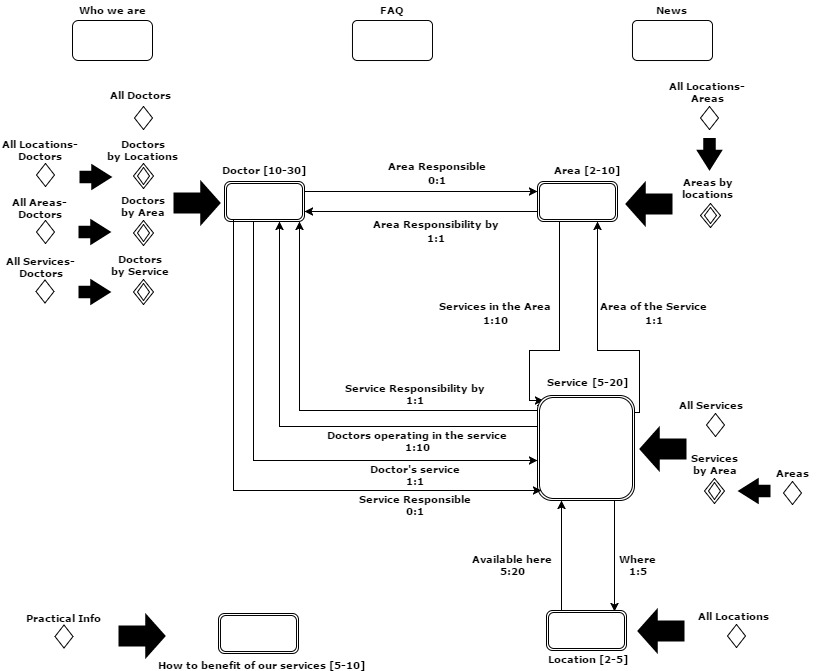
\includegraphics[width=\textwidth]{Clinic_C_IDM.jpg}
\end{center}}

\newpage

{\centering 
L-IDM Schema
\vspace{1cm}
\begin{center}
	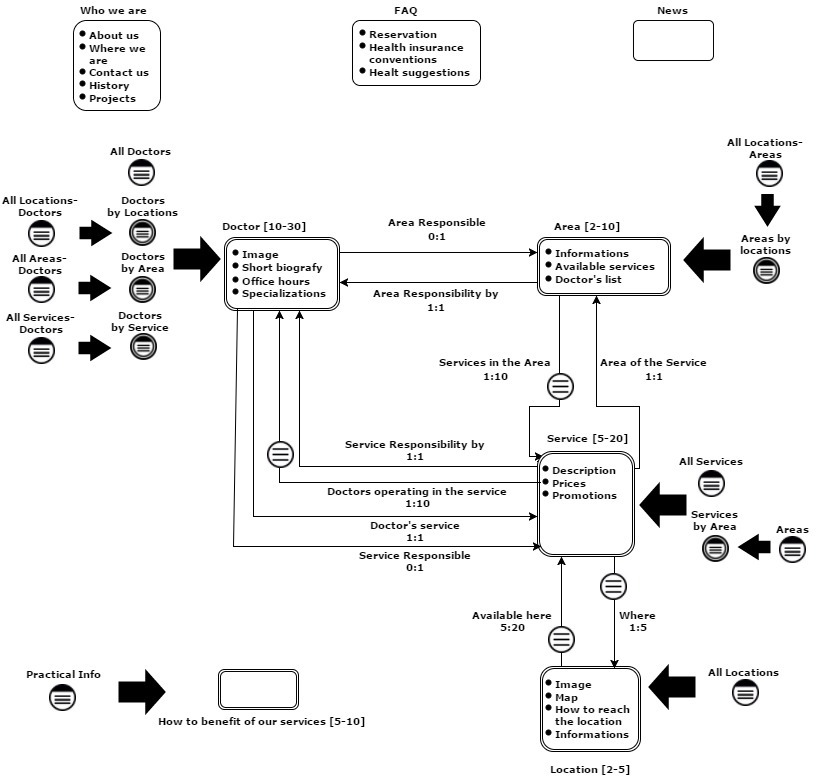
\includegraphics[width=\textwidth]{Clinic_L_IDM.jpg}
\end{center}}

\newpage

{\centering 
P-IDM Schema
\vspace{1cm}
\begin{center}
	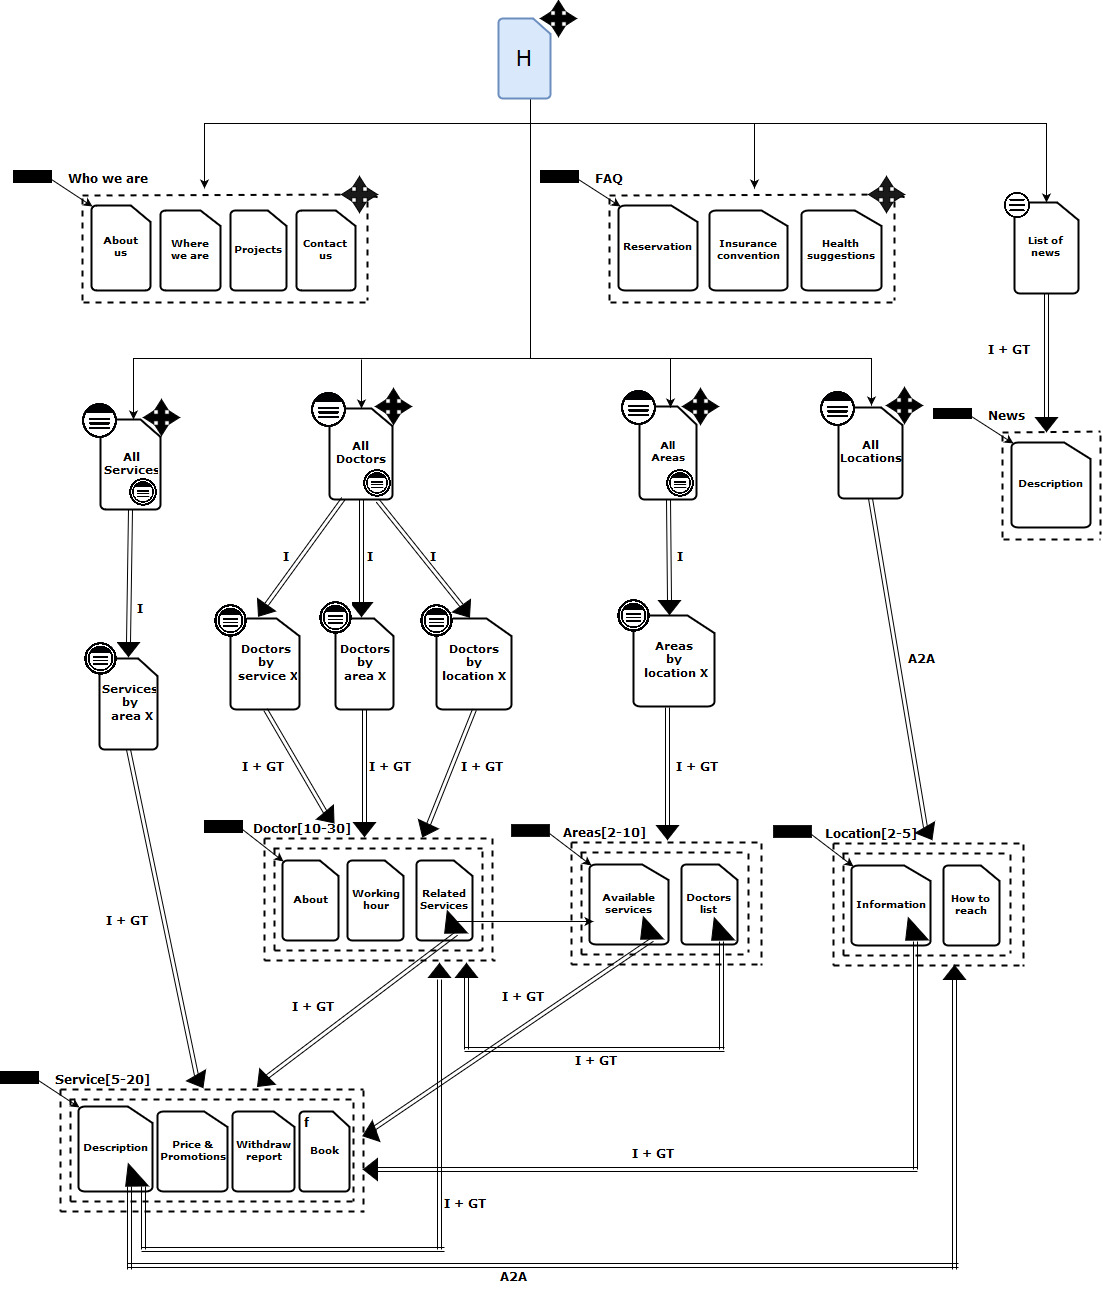
\includegraphics[width=\textwidth]{Clinic_P_IDM.jpg}
\end{center}}


\chapter{Scenarios}
\thispagestyle{fancy}
\section{Scenario 1}
Bob ha bisogno di effettuare un elettrocardiogramma. Diverse persone gli hanno suggerito  di effettuarla all' Hospidif.
Bob non è mai stato nella clinica e quindi prima di tutto decide di informarsi meglio a riguardo accedendo al portale www.hospidif.com
Dalla homepage clicca sul pulsante Services. A questo punto gli viene richiesto di selezionare un area sulla quale filtrare i servizi.
Quindi clicca sull'area cardiologia. Tra i vari servizi sceglie elettrocardiogramma e accede alla pagina contenente tutte le informazioni
riguardanti il servizio. Leggendo la descrizione del servizio nota che c'è solo una location nel quale viene effettuato il
servizio quindi clicca sul link "London Westmister". Legge le informazioni della location e cliccando sul pulsante "How to reach the location"
scoprendo che non è molto distante dalla propria abitazione. A questo punto, quindi, decide di informarsi meglio e torna indietro nella pagina
di descrizione del servizio e questa volta clicca sul primo dottore della lista. Bob si trova,dunque, nella pagina di descrizione del dottore 
e legge tutte le informazioni riguardanti il curante. Ripete il passaggio con tutti i dottori nella lista. A questo punto Bob, sempre
più interessato alla clinica decide di contattare il responsabile dell'area di riferimento in modo da prendere un appuntamento.
Dunque clicca sul bottone "Areas" nel quale gli viene richiesto di scegliere la location sula quale filtrare le aree. Seleziona London Westmister e,
successivamente, seleziona "Cardiology" e clicca sul dottore responsabile. Clicca sul pulsante Call e ottiene il suo numero di telefono.

\newpage

\section{Scenario 2}
Patrick ha da pochi giorni usufruito di un servizio dell'Hospidif. Dato che è molto soddisfato di come è stato trattato dalla clinica decide di accedere
sul sito per leggere un po di informazioni a riguardo. Dalla homepage clicca sul bottone "Who we are" e legge tutte le info riguardo la storia della clinica.
Successivamente clicca sul bottone projects per leggere info su tutti i progetti sui quali la clinica sta lavorando. Successivamente clicca sul bottone "news"
in alto nella pagina. A questo punto si trova davanti una lista di news e, molto interessato ad una in particolare clicca su di essa andando a leggere tutte le
informazioni a riguardo.

\newpage

\section{Scenario 3}


\chapter{Wireframes}
\thispagestyle{fancy}
\foreach\x in {1,5,6,7,29,41,75,76,119,120,148,158,117,184,186,189,198,200,204,207,212}{
	\begin{center}
		\includegraphics[page=\x, width=\textwidth]{../Mockup/Desktop/mockup2.pdf}
	\end{center}
	\vspace{0.7cm}
}

\appendix
\chapter{Appendix}
\section{Version History}
In the following are listed the differences between versions:
\begin{itemize}
	\item 1.0.0: first release
\end{itemize}
\end{document}
